

\section{Datensynchronisation mit REST-Schnittstelle} 

\subsection{Datensynchronisation}

Nachdem die Messwerte aufgezeichnet sind, werden sie dem Arzt zug\"anglich gemacht.
So macht sich der Arzt ein Bild vom Zustand des Patienten und stellt eine Diagnose.
F\"ur diesen Zweck werden die Messprotokolle an einen Webserver gesendet.
Das Senden oder Synchronisieren startet immer wenn eine Activity beendet werden soll.
Als Beispiel wird die Activity f\"ur die Blutdruckmessung n\"aher betrachtet.
Damit das GUI nicht blockiert wird, muss das Synchronisieren immer nebenl\"aufig geschehen.
F\"ur diesen Zweck wird eine Klasse vom Typ AsyncTask genutzt.
Ein AsyncTask ist in drei Arbeitsbereiche aufgeteilt.
Im ersten Arbeitsbereich wird die Aufgabe noch im UI-Thread ausgef\"uhrt.
Daf\"ur ruft er seine Methode \emph{onPreExecute()} auf.
Hier kann der AsyncTask noch direkt auf die Activity zugreifen und die Aufgabe vorbereiten.
Im n\"achsten Schritt startet der AsyncTask einen eigenen Thread und f\"uhrt
die Aufgabe nun in seine \emph{doInBackground()}-Methode aus.
Das ist der nebenl\"aufige Teil der Ausf\"uhrung.
Ist dieser beendet, wird die Methode \emph{onPostExecute()} aufgerufen.
Er befindet sich wieder im UI-Thread.
Bevor ein AsyncTask beendet wird, werden hier noch die Ergebnisse an die Activity \"ubergeben.
Das Listing 4.9 zeigt eine reduzierte Form der \emph{SynchronizeBloodpressure}-Klasse, welche die Klasse
AsyncTask erweitert.
Die Messwerte werden mit einem AsyncTask gesendet.
Zuerst wird die Netzwerk- und Serververf\"ugbarkeit gepr\"uft.
Schl\"agt der Test fehl, so wird die Ausf\"uhrung beendet.
Als n\"achstes werden JSON-Objekte erzeugt, in denen die Messdaten abgelegt werden.
Im n\"achsten Schritt werden Tagesprotokolle, die noch nicht synchronisiert wurden, aus der Datenbank gelesen und
in JSON-Objekte gepackt.
Danach wird die URL zum Webserver zusammengebaut.
Dieser Vorgang ist wichtig, da zwar immer dieselbe IP genutzt wird, aber f\"ur jede Aufgabe wird ein anderes 
PHP-Skript vom Server aufgerufen.
Die PHP-Skripte bilden eine REST-Schnittstelle f\"ur die ApoCo-Anwendung.
Nachdem die URL bereitgestellt ist, wird eine Verbindung zum Webserver aufgebaut und ein 
\emph{HTTPRequest} ausgef\"uhrt.
Dabei werden die JSON-Strings mitgesendet.
Im letzten Schritt wird die Antwort vom Server ausgewertet und der 
Synchronisationsvorgang in der lokalen Datenbank best\"atigt.
Dabei wird das \emph{Sync}-Flag jeder synchronisierten Messung in der lokalen Datenbank auf den 
Wert 1 gesetzt und eine R\"uckmeldung an die Activity ausgegeben.
Der Synchronisationsvorgang wird in Abbildung 4.10 veranschaulicht.\\

\begin{figure}[h]
  \centering
  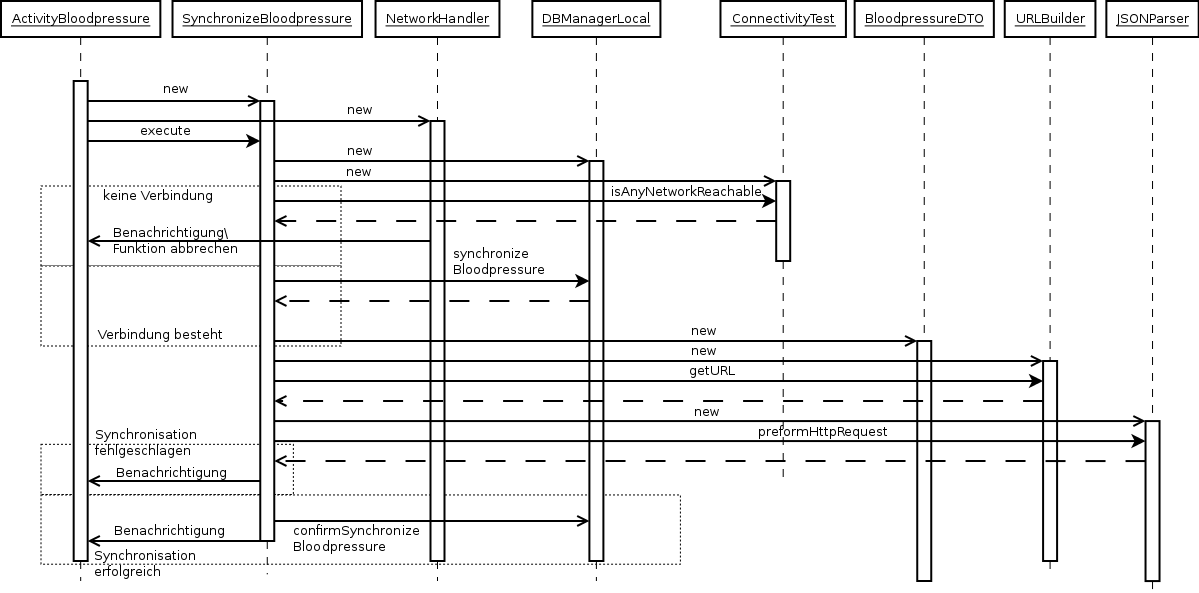
\includegraphics[scale=0.36]{diagramme/kapitel4/sequenzdiagramme/data_sync.png}
  \caption{Sequenzdiagramm f\"ur das Senden der Tagesprotokolle an den Webserver}
  
\end{figure}

\begin{lstlisting}[caption={SynchronizeBloodpressure sendet Blutdruckmesswerte an den Webserver}]
public class SynchronizeBloodpressure extends AsyncTask<UserDTO, Void, Boolean> {

   protected void onPreExecute() {
      ... /*Ablauf im UI-Thread*/
   } 
   /*ab hier startet ein neuer Thread*/
   protected Boolean doInBackground(UserDTO... pUser) {
      //Netzwerkverfuegbarkeit pruefen
      isNetworkConnected = new ConnectivityTest(mContext).isAnyNetworkReachable(mHandlerNet);
      if (!isNetworkConnected) return false;
      mUser = pUser[0];
      //JSON-Strukturen zum Senden werden angelegt
      JSONObject user = mUser.toJSONObject();
      JSONArray payload = new JSONArray();
      try {
         //Daten zum Synchronisieren aus der Datenbank laden
         Cursor cursor = mDBManager.synchronizeBloodpressure(mUser);
         while (cursor.moveToNext()) {
            //Daten in JSON-Strings verpacken
            BloodpressureDTO bpdto = new BloodpressureDTO(cursor);
            payload.put(cursor.getPosition(), bpdto.toJSONObject());
         }
      } catch (JSONException e) {}
      List<NameValuePair> params = new ArrayList<NameValuePair>();
      //JSON-String als Parameter fuer die Uebergabe an eine URL vorbereiten
      params.add(new BasicNameValuePair(JSON_TAG_IF.USER, user.toString()));
      params.add(new BasicNameValuePair(JSON_TAG_IF.PAYLOAD, payload.toString()));
      //aus Konfigurationsdaten die URL zusammenbauen
      String url = new URLBuilder().getURL(mContext, PHP_URL_IF.INSERT_BLOODPRESSURE);
      //HTTP-Anfrage an den Webserver senden
      jsonObject = new JSONParser().preformHttpRequest(url, JSONParser.RequestMethodE.POST, params);		
      try {
         //Antwort vom Webserver lesen
         int success = jsonObject.getInt(JSON_TAG_IF.SUCCESS);
         if (1 == success) {... return true;}
         else { return false;}
      }
    //Ende der Ausfuehrung, jetzt wieder im UI-Thread
    protected void onPostExecute(Boolean result) {
       if (result) {
       } else {
          //Nachricht kann direkt an die Activity uebergeben werden, hier geschieht es ueber ein Handler
          mHandlerAct.obtainMessage(ActivityBloodpressure.SYNCHRONIZING_DATA_COMPLETE).sendToTarget();
       }
       progressDialog.dismiss();
    }
}
\end{lstlisting}

\subsection{REST-Schnittstelle}

Die Rest-Schnittstelle auf dem Webserver ist aus mehreren PHP-Skripten aufgebaut.
Es gibt pro Funktionalit\"at ein Skript.
Die Persistenzschicht ist auf dem Webserver identisch modelliert, wie das in der Android-Anwendung der Fall ist.
Daf\"ur gibt es f\"ur jede Tabelle in der Datenbank eine entsprechende \emph{COLUMNS-, DTO-} und \emph{TBL-}Klasse.
Diese Klassen haben die gleiche Funktionalit\"at wie in der Android-Anwendung.
Sie beschreiben die Struktur und Tabellen der Datenbank als Objekte.
F\"ur die Verwaltung der Persistenzschicht ist die Klasse \emph{\texttt{DB\_Manager}} verantwortlich.
Dieser Manager baut bei Bedarf eine Verbindung zur Zieldatenbank auf und leitet die Anfragen an sie weiter.
Hier werden zwei unterschiedliche Datenbanken verwendet.
Eine geh\"ohrt zum Projekt \emph{ClearFood}.
Dort werden Informationen \"uber die Lebensmittel abgefragt.
Die andere Datenbank geh\"ohrt zu der Android-Anwendung ApoCo.
Hier werden die Messprotokolle aller Patienten gespeichert.
Wie eine Verbindung zur Datenbank gemacht wird, veranschaulicht das Listing 4.10.
Hier wird zum Aufbau der Kommunikation die Methode \emph{connect()} der Klasse \emph{\texttt{DB\_Manager}} gerufen.
Da die meisten Anfragen an die ApoCo-Datenbank gerichtet sind, 
wird hier standardm\"a\ss{}ig die Verbindung zu dieser Datenbank aufgebaut.\\

\begin{lstlisting}[caption={Verbindungsaufbau zur Datenbank}]
class DB_Manager {   
   private $db;   
   function connect() {
      $this->db = new mysqli(SERVER, USER, PASSWORD, DATABASE);
      return $this->db;
   }
}
//Verbindungsaufbau
$db = new DB_Manager();
$db->connect();
\end{lstlisting}

Die Anfragen sendet ApoCo an den Webserver \"uber HTTP.
Dabei wird f\"ur die gew\"unschte Anfrage ein PHP-Skript aufgerufen.
Eine solche Anfrage wird hier am Beispiel der Registrierung eines neuen Patienten im System veranschaulicht.
F\"ur das Registrieren wird das Skript \emph{register\texttt{\_}user.php} benutzt.
Der erste Schritt wird im Listing 4.11 demonstriert. 
Hier wird ein Array mit der Bezeichnung \emph{response} und ein Objekt der 
Klasse \emph{DB\texttt{\_}Manager} erstellt.
Das Array wird f\"ur die Antwort vom Server an die Android-Anwendung genutzt.\\

\begin{lstlisting}[caption={Benuzter registrieren, Schritt 1}]
$response = array();
$db = new DB_Manager();
\end{lstlisting}

Die Kommunikation zwischen ApoCo und Webserver wird hier durchgehend \"uber die HTTP-Methode POST gemacht.
Im n\"achsten Schritt werden mit der Funktion \emph{checkPOSTValues()} die Parameter in der 
Variablen POST auf G\"ultigkeit \"uberpr\"uft.
Die Methode \emph{checkPOSTValues()} wird im Listing 4.12 demonstriert.
Sind die empfangenen Parameter in Ordnung, wird die Abfrage ausgef\"uhrt.
Hat der Test fehlgeschlagen, wird eine entsprechende Nachricht als JSON-String zur\"uck an den Aufrufer gesendet.\\

\begin{lstlisting}[caption={Benuzter registrieren, Schritt 2}]
if (checkPOSTValues()) {
   //ok
} else {
   $response["success"] = 0;
   $response["message"] = "required field(s) is missing";
   echo json_encode($response);
}

function checkPOSTValues() {
   return isset($_POST[UserColumns::VORNAME]) &&
   isset($_POST[UserColumns::NACHNAME]) &&
   isset($_POST[UserColumns::EMAIL]) && 
   isset($_POST[UserColumns::PASSWORD]);
}
\end{lstlisting}

Sind die Parameter akzeptiert, so geht es mit dem n\"achsten Schritt weiter.
Mit der Klasse \emph{UserDto} wird aus den Parametern ein User-Objekt erzeugt.
Anschlie\ss{}end wird eine Verbindung zur Datenbank ge\"offnet.
Es wird gepr\"uft, ob die Email des neuen Benutzers bereits in der Datenbank vorhanden ist.
Ist das der Fall, wird seine Registrierung abgelehnt.
Handelt es sich dabei um keine bekannte Email, wird der neue Benutzer in die Datenbank aufgenommen 
und eine entsprechende positive R\"uckmeldung an den Aufrufer gesendet.
Diesen Vorgang veranschaulicht das Listing 4.13.\\

\begin{lstlisting}[caption={Benuzter registrieren, Schritt 3}]
$user = new UserDto($_POST);
$db->connect();
if($db->emailInUse($user->getEmail()) == 0) {
   $result = $db->registerNewUser($user);
   if($result) {
      $response["success"] = 1;
      $response["message"] = "user successfully registered";
      echo json_encode($response);
   } else {
      $response["success"] = 0;
      $response["message"] = "user registering failed";
      echo json_encode($response);
   }
} else { 
   $response["success"] = 0;
   $response["message"] = "email <" . $user->getEmail() . "> allready in use";
   echo json_encode($response);
}
\end{lstlisting}